\chapter{Risultati}

L'intervista è stata inviata a 60 infermieri: 9 non hanno partecipato, quindi in totale sono stati raccolti 51 questionari. Gli infermieri che hanno preso parte allo studio lavorano nei seguenti reparti: 18 in Clinica Pediatrica, 13 nel servizio di Day Hospital Pediatrico, 13 nella struttura di Oncoematologia, 5 in quella di Ortopedia e Traumatologia e 2 in quella di Radiologia Pediatrica - servizio di Risonanza Magnetica. Gli anni di esperienza degli intervistati variano da 6 mesi a 36 anni, con una mediana di 10 anni (IQR 2-22.75). 27 infermieri (53$\%$) assistono meno di 10 sedazioni procedurali al mese, 14 (27.4$\%$) da 10 a 20, 8 (15.7$\%$) da 21 a 30 e 2 (3.9$\%$) più di 30 sedazioni ogni mese. 32 partecipanti hanno dato un punteggio di soddisfazione della qualità globale della sedazione effettuata con il propofol in scala numerica da 0 a 10 (\texttt{NRS}) $\geq$8 

\begin{figure}[h]
    \centering
    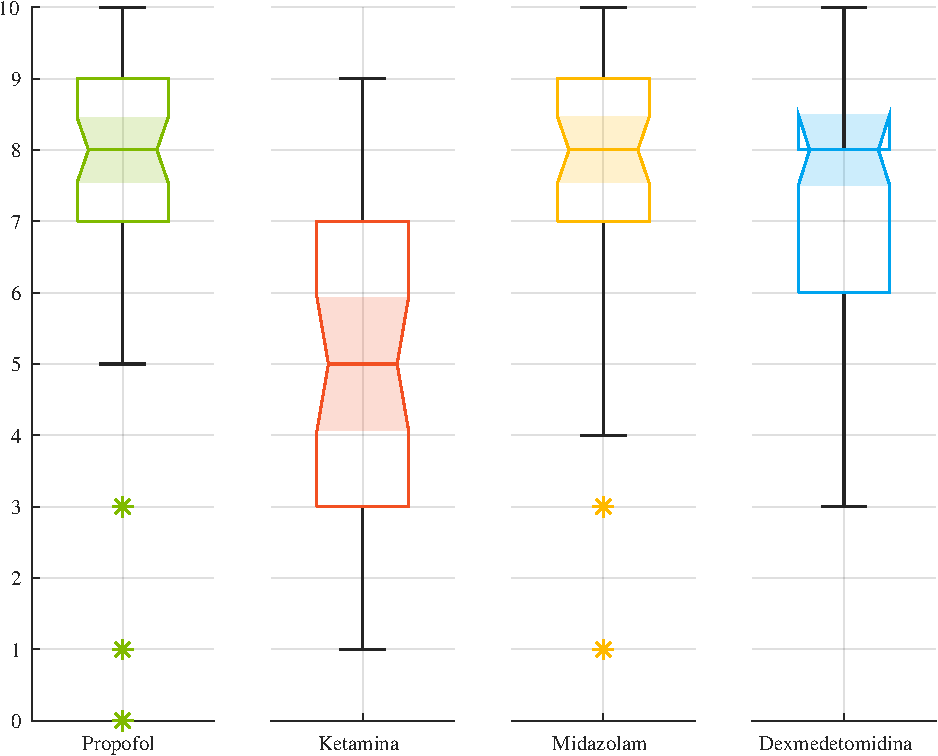
\includegraphics[width=0.8\textwidth]{Figure/qualita-colorful.pdf}
    \caption{Confronto del livello di soddisfazione percepito dagli infermieri (misurato in scala NRS) in relazione ai quattro agenti farmacologici testati in questo lavoro di tesi.}
    \label{fig:qualitascolorful}
\end{figure}

\begin{figure}[h]
    \centering
    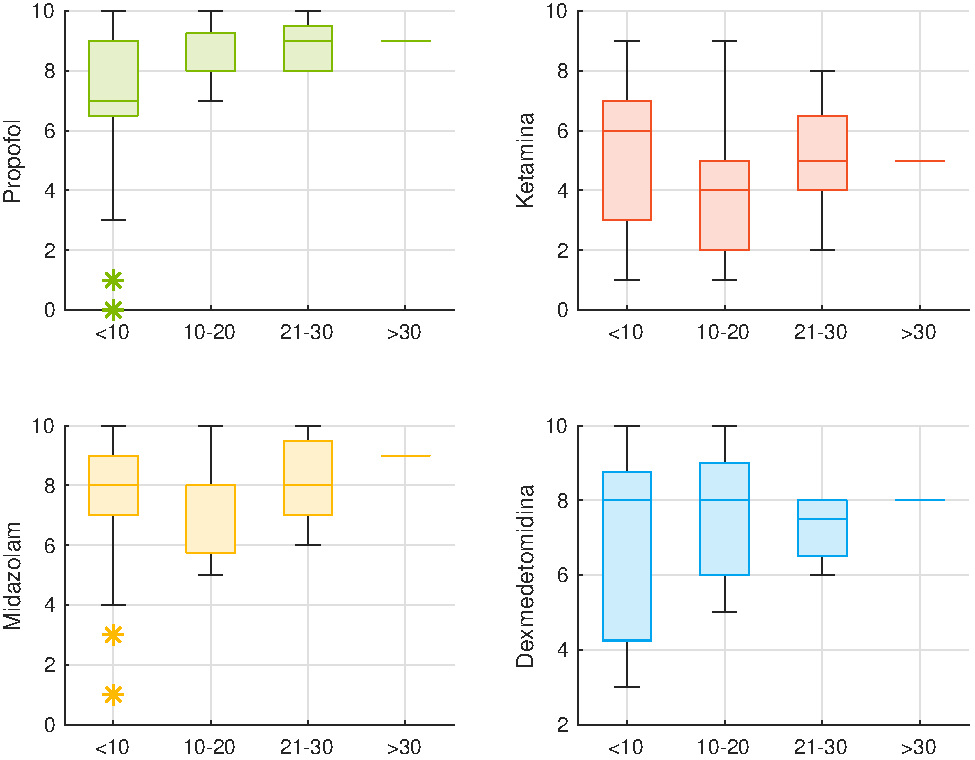
\includegraphics[width=1\textwidth]{Figure/qualita-stratificata.pdf}
    \caption{Livello di soddisfazione associato ai diversi agenti farmacologici (misurato secondo scala NRS) stratificato per il numero di sedazioni mensilmente assistite dagli intervistati.}
    \label{fig:qualitastratificata}
\end{figure}